\chapter{Results and Discussion}
\label{Results}

\section{Model Performance}

The performance of each machine learning model on each dataset is presented in the following tables. The classification accuracy on the training set, as well as the classification accuracy, precision, recall, F1 score, and ROC AUC on the test set, are reported. All values are reported as percentages unless otherwise indicated. The best result achieved for each metric is highlighted in \textbf{bold}.

\subsection{Full dataset}

The full dataset consists of 10145 matches, with 8116 used for training and 2029 for testing. Each model was first trained using all 142 features. The results obtained for this setup are tabulated in Table \ref{table:1}.

\begin{table}[h!]
	\centering
	\small
	\begin{adjustbox}{center} % Center the table
		\begin{tabular}{ |l|c|c|c|c|c|c| }
			\hline
			\rule{0pt}{2.6ex} \textbf{Model} & \textbf{Train ACC} & \textbf{Test ACC} & \textbf{Precision} & \textbf{Recall} & \textbf{F1 Score} & \textbf{ROC AUC} \\
			\hline
			\rule{0pt}{2.6ex} TrueSkill                 & 56.8 & 57.9 & 57.2 & 62.4 & 59.7 & 61.6 \\ \hline
			\rule{0pt}{2.6ex} Logistic Regression 		& 60.0 & 58.5 & 56.9 & 69.3 & 62.5 & 62.9 \\
			\rule{0pt}{2.6ex} Random Forest 			& 64.3 & 58.3 & 56.7 & 69.9 & 62.6 & 62.5 \\
			\rule{0pt}{2.6ex} Support Vector Machine 	& 59.5 & 59.4 & \textbf{58.3} & 66.3 & 62.0 & 63.0 \\
			\rule{0pt}{2.6ex} XGBoost 					& 61.0 & \textbf{60.0} & \textbf{58.5} &\textbf{ 69.6} & \textbf{63.5} & \textbf{64.1} \\
			\rule{0pt}{2.6ex} Gaussian Naive Bayes 		& 56.6 & 55.7 & 57.4 & 44.5 & 50.1 & 59.0 \\
			\rule{0pt}{2.6ex} MLP Neural Network 		& 59.9 & 59.7 & 59.0 & 63.8 & 61.3 & 62.1 \\
			\rule{0pt}{2.6ex} k-Nearest Neighbours 		& 58.9 & 55.9 & 55.3 & 61.2 & 58.1 & 57.8 \\
			\hline
		\end{tabular}
	\end{adjustbox}
	\caption{Performance of ML models trained with all features on complete dataset}
	\label{table:1}
\end{table}

The ML models did not significantly outperform the TrueSkill baseline model, with the improvement in classification accuracy varying from -2\% to 2\%. XGBoost and MLP had the best overall performance with a classification accuracy of 60.0\% and 59.7\%  respectively. XGBoost had the highest recall, $F_1$ score, and AUC ROC, indicating slightly better ability to discriminate between classes.

The optimal set of hyperparameters for each model was found using grid search and is captured in Table \ref{table:hyperparameters} below.

 \begin{table}[h]
	\centering
	\small
	\begin{adjustbox}{center}
		\begin{tabular}{|l|l|l|}
			\hline
			\rule{0pt}{2.5ex}\textbf{Hyperparameter} & \textbf{Description} & \textbf{Value Selected} \\
			\hline
			\multicolumn{3}{|c|}{\rule{0pt}{2.5ex}\textit{Logistic Regression}} \\
			\hline
			C & Inverse of regularization strength & 0.01 \\
			penalty & Type of regularization & "l2" \\
			solver & Optimization algorithm & "liblinear" \\
			\hline
			\multicolumn{3}{|c|}{\rule{0pt}{2.5ex}\textit{Random Forest}} \\
			\hline
			n\_estimators & Number of trees in the forest & 100-400 \\
			max\_depth & Maximum depth of the tree & 2 \\
			min\_samples\_split & Min samples to split a node & 4 \\
			min\_samples\_leaf & Min samples to be at a leaf node & 4 \\
			max\_features & Number of features for best split & "log2" \\
			\hline
			\multicolumn{3}{|c|}{\rule{0pt}{2.5ex}\textit{Support Vector Machine}} \\
			\hline
			C & Regularization parameter & 0.1 \\
			kernel & Kernel type & "linear" \\
			gamma & Kernel coefficient & "scale" \\
			\hline
			\multicolumn{3}{|c|}{\rule{0pt}{2.5ex}\textit{XGBoost}} \\
			\hline
			n\_estimators & Number of gradient boosted trees & 208 \\
			learning\_rate & Step size shrinkage & 0.025 \\
			max\_depth & Maximum depth of a tree & 2 \\
			subsample & Subsample ratio of the training instances & 0.5 \\
			colsample\_bytree & Subsample ratio of columns for each tree & 0.5 \\
			gamma & Min loss reduction for partition on a leaf node & 0.1 \\
			\hline
			\multicolumn{3}{|c|}{\rule{0pt}{2.5ex}\textit{Gaussian Naive Bayes}} \\
			\hline
			var\_smoothing & Variance smoothing & 1e-9 \\
			\hline
			\multicolumn{3}{|c|}{\rule{0pt}{2.5ex}\textit{Multi-layer Perceptron}} \\
			\hline
			hidden\_layer\_sizes & Neurons in hidden layers & (5,4) \\
			activation & Activation function & "relu" \\
			solver & Solver for weight optimization & "sgd" \\
			alpha & L2 penalty (regularization term) & 0.001 \\
			learning\_rate & Learning rate for weight updates & "constant" \\
			\hline
			\multicolumn{3}{|c|}{\rule{0pt}{2.5ex}\textit{k-Nearest Neighbours}} \\
			\hline
			n\_neighbors & Number of neighbors to use & 110 \\
			weights & Weight function in prediction & "uniform", "distance" \\
			algorithm & Algorithm to compute nearest neighbors & "auto" \\
			p & Power parameter for Minkowski metric & 1 (Manhattan) \\
			\hline
		\end{tabular}
	\end{adjustbox}
	
	\caption{Hyperparameters and range of values tested for each ML model implemented}
	\label{table:hyperparameters2}
\end{table}

% LOG {'C': 0.01, 'penalty': 'l2', 'solver': 'liblinear'}
% RAN {'criterion': 'gini', 'max_depth': 5, 'max_features': 'log2', 'min_samples_leaf': 4, 'min_samples_split': 4, 'n_estimators': 300}
% SVM {'C': 0.1, 'gamma': 'scale', 'kernel': 'linear'}
% XGB {'learning_rate': 0.025, 'max_depth': 2, 'n_estimators': 200}
% GNV {'var_smoothing' : '1e-09'}
% MLP {'activation': 'relu', 'alpha': 0.001, 'hidden_layer_sizes': (10,100,10), 'learning_rate_init': 0.001, 'solver': 'sgd'}
% KNN {'n_neighbors': 110, 'p': 1, 'weights': 'uniform'}

As a consequence of the large number of features, the models were prone to overfit the training data. This was especially pronounced with random forests, XGBoost, and MLP, which when initially configured could achieve near perfect accuracy on the training set, but otherwise performed poorly on the test set. In the case of random forests and XGBoost, this was mitigated by reducing the maximum depth of the trees to only 2 splits. For MLP, the number of nodes per hidden layer had to be quite low (5,4) to avoid overfitting.

The weakest performers were $k$-nearest neighbours and Gaussian Naive Bayes, exhibiting worse performance than the TrueSkill base model.

The ROC curve for TrueSkill and the best performing ML model, XGBoost, are plotted in Figure \ref{fig:xgb-roc}. It is evident that both models are better at predicting match outcomes than random chance, however XGBoost is slightly superior with an AUC of 0.641 vs 0.624.

\begin{figure}[h]
	\centering
	\begin{adjustbox}{center}
		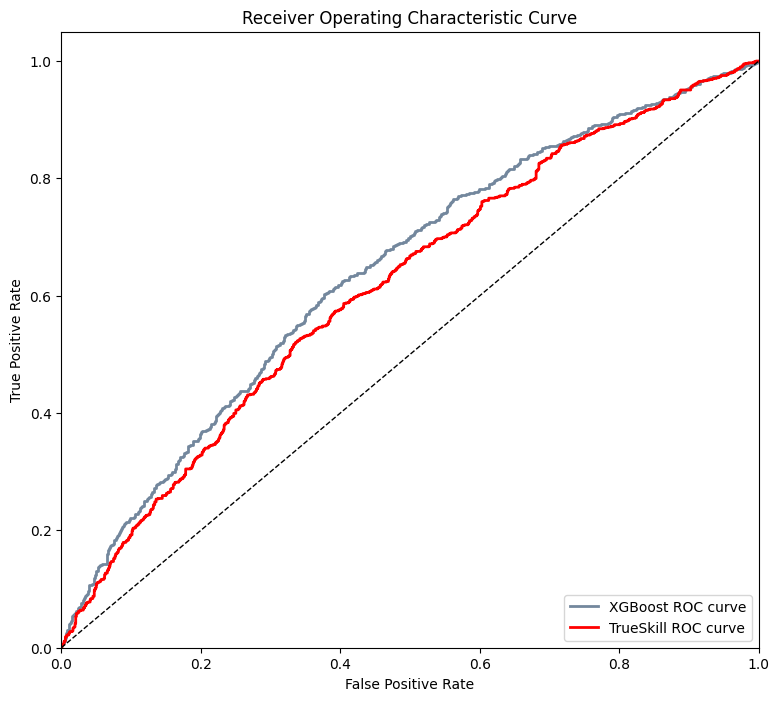
\includegraphics[width=1.1\textwidth]{Figures/xgb-auc.png}
	\end{adjustbox}
	\caption{Receiver operating characteristic curve for TrueSkill and XGBoost}
	\label{fig:xgb-roc}
\end{figure}

\subsubsection{Feature importance}

Feature selection methods such as filter and wrapper methods have already been discussed in section \ref{feature-selection}. Some models can also be used to determine feature importance. In a regularised logistic regression model, the magnitude of the coefficients for each feature are indicative of their importance given a large enough regularization penalty. 

For SVMs with linear kernels, the weights assigned to each feature indicate their importance. With tree-based methods like random forests and XGBoost, the features yielding the largest average reduction in the loss function are more important. Figure \ref{fig:xgbimp} shows the feature importances determined by XGBoost.

\begin{figure}[h]
	\centering
	\begin{adjustbox}{center}
		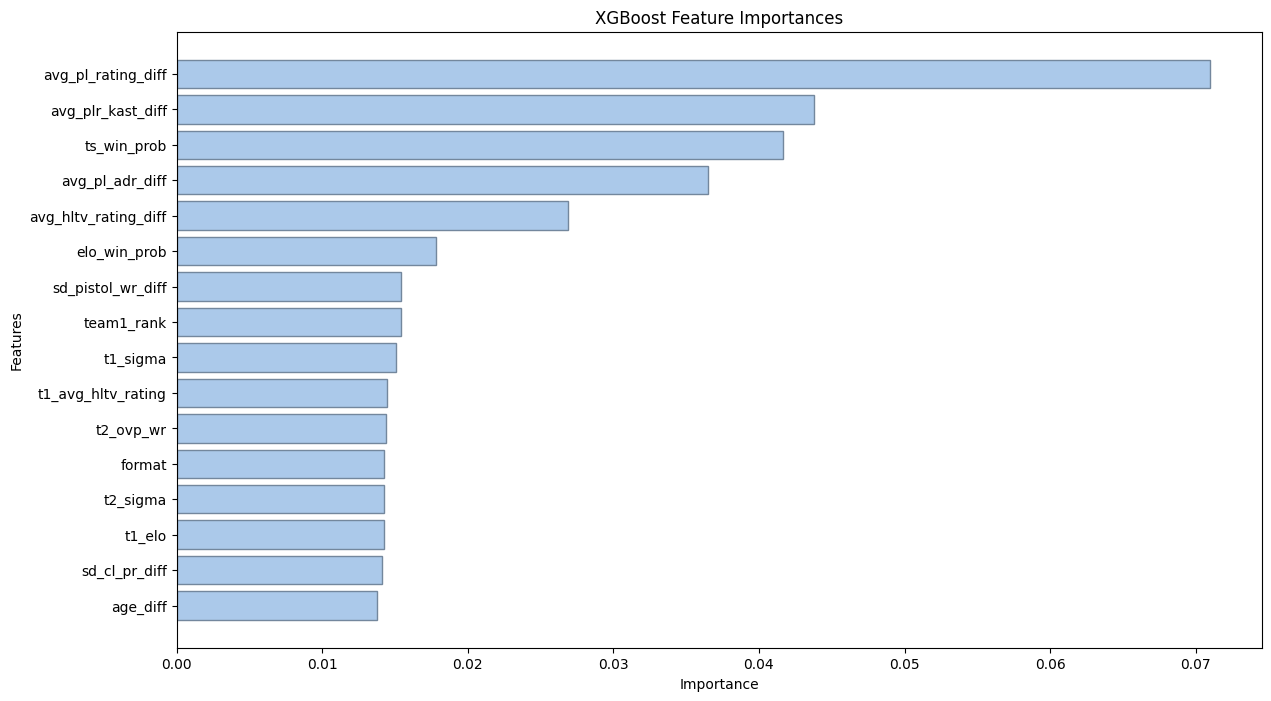
\includegraphics[width=1.3\textwidth]{Figures/xgb-imp.png}
	\end{adjustbox}
	\caption{Feature importance from XGBoost}
	\label{fig:xgbimp}
\end{figure}

In contrast to the filter methods in section \ref{feature-selection}, XGBoost considers the difference in average player statistics (rating, KAST, ADR, and HLTV rating) between the two teams to be highly relevant measures. Both TrueSkill and Elo win probabilities are taken into account as well, whereas previously the Elo measure was discarded. 

With logistic regression, the feature importances differed considerably. As seen in Figure \ref{fig:logimp}, the TrueSkill win probability and $\mu,\sigma$ values for either team were very important, followed by the difference in average map win-rate, round win-rate per map. HLTV world ranking, and win-streak.

\clearpage

\begin{figure}[h]
	
	\centering
	\begin{adjustbox}{center} % Center the table
		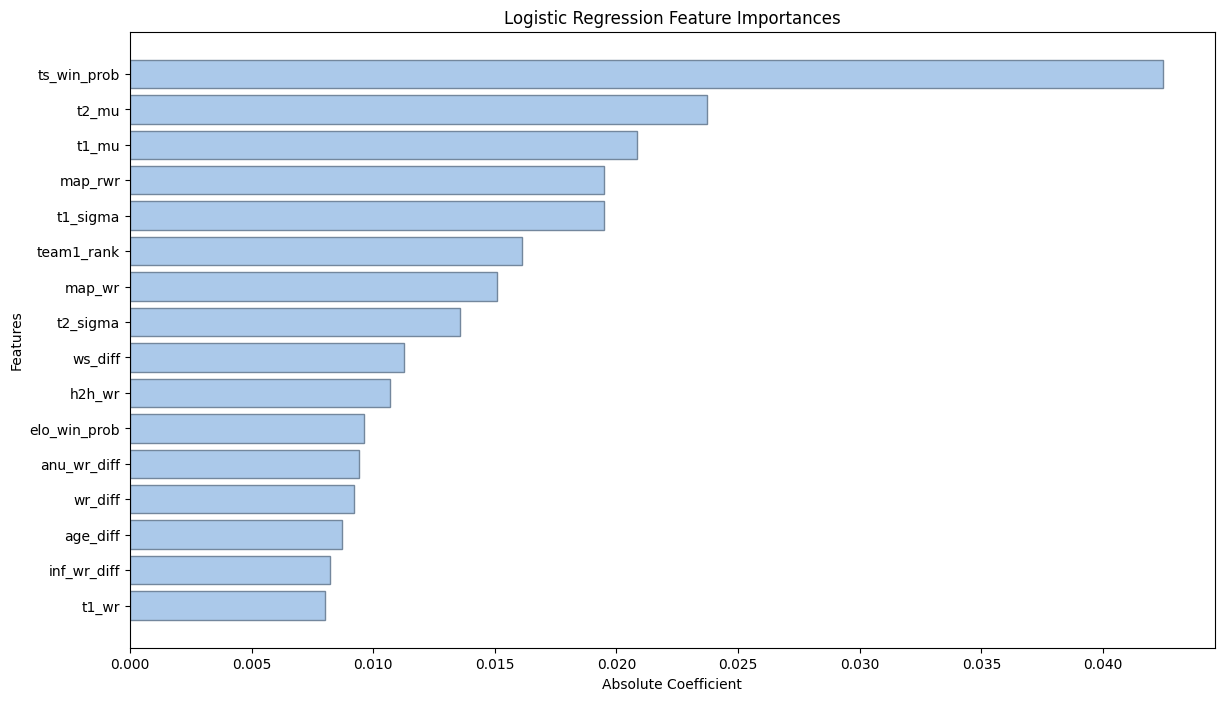
\includegraphics[width=1.3\textwidth]{Figures/logreg-imp.png}
	\end{adjustbox}
	\caption{Feature importance from logistic regression coefficients}
	\label{fig:logimp}
\end{figure}

The results reported in Table \ref{table:2} below were obtained after reducing the number of features to 18, an 87\% reduction in the data provided to each model. This smaller set of features was determined using the list of feature importance graphs produced from the previous analysis. The number of matches in the training and testing sets remained the same.

\begin{table}[h!]
	\centering
	\small
	\begin{adjustbox}{center} % Center the table
		\begin{tabular}{ |l|c|c|c|c|c|c| }
			\hline
			\rule{0pt}{2.6ex} \textbf{Model} & \textbf{Train ACC} & \textbf{Test ACC} & \textbf{Precision} & \textbf{Recall} & \textbf{F1 Score} & \textbf{ROC AUC} \\
			\hline
			\rule{0pt}{2.6ex} TrueSkill                 & 56.8 & 57.9 & 57.2 & 62.4 & 59.7 & 61.6 \\ \hline
			\rule{0pt}{2.6ex} Logistic regression 		& 58.4 & 59.1 & 57.7 & 67.7 & 62.3 & 62.2 \\
			\rule{0pt}{2.6ex} Random forests 			& 63.3 & 59.1 & 57.7 & 68.3 & 62.5 & 63.3 \\
			\rule{0pt}{2.6ex} Support vector machine 	& 59.7 & 57.4 & 55.6 & \textbf{74.0} & \textbf{63.5} & 62.8 \\
			\rule{0pt}{2.6ex} XGBoost 					& 60.0 & 59.3 & 57.9 & 68.6 & 62.8 & \textbf{64.2} \\
			\rule{0pt}{2.6ex} Gaussian Naive Bayes 		& 58.3 & 57.9 & 56.9 & 65.2 & 60.8 & 61.0 \\
			\rule{0pt}{2.6ex} Multilayer perceptron     & 59.8 & \textbf{59.8} & \textbf{58.6} & 66.4 & 62.3 & 63.7 \\
			\rule{0pt}{2.6ex} $k$-nearest neighbours 	& 63.9 & 53.9 & 53.4 & 60.6 & 56.7 & 55.8 \\
			\hline
			\rule{0pt}{2.6ex} \textbf{Mean Change} 		& +0.45 & -0.12 & -0.59 & +3.74 & +1.54 & +0.23 \\
			\hline
		\end{tabular}
	\end{adjustbox}
	\caption{Performance of ML models trained with 18 selected features on the complete dataset}
	\label{table:2}
\end{table}

% XGBoost: {'colsample_bytree': 1, 'learning_rate': 0.08, 'max_depth': 1, 'n_estimators': 208, 'subsample': 0.7}

The reduction in the number of features did not significantly degrade performance. In fact, the Recall, $F_1$ score, and ROC AUC all increased on average - likely due to a reduction in noise. This strongly suggests that many of the features do not meaningfully contribute to an accurate match prediction and can safely be ignored.

Occam's razor recommends searching for an explanation constructed from the smallest possible set of elements. This begs the question: how many features can be removed from the dataset without incurring a considerable loss in performance? 

Another test was performed by reducing the total number of features to just seven features: difference in average player rating, TrueSkill win probability and both teams' $\mu$-values, the difference in their HLTV world ranking, the first team's HLTV world ranking, and the number of maps where the first team had a higher round win-rate than their opponent. The results are shown below in Table \ref{table:7features}.

\begin{table}[h!]
	\centering
	\small
	\begin{adjustbox}{center} % Center the table
		\begin{tabular}{ |l|c|c|c|c|c|c| }
			\hline
			\rule{0pt}{2.6ex} \textbf{Model} & \textbf{Train ACC} & \textbf{Test ACC} & \textbf{Precision} & \textbf{Recall} & \textbf{F1 Score} & \textbf{ROC AUC} \\
			\hline
			\rule{0pt}{2.6ex} TrueSkill                 & 56.8 & 57.9 & 57.2 & 62.4 & 59.7 & 61.6 \\ \hline
			\rule{0pt}{2.6ex} Logistic regression 		& 57.7 & 58.8 & 58.0 & 63.6 & 60.7 & 61.1 \\
			\rule{0pt}{2.6ex} Random forests			& 62.1 & 59.0 & 57.6 & \textbf{67.9} & 62.3 & 62.3 \\
			\rule{0pt}{2.6ex} Support vector machine 	& 57.5 & 58.7 & 57.7 & 65.1 & 61.2 & 61.8 \\
			\rule{0pt}{2.6ex} XGBoost 					& 59.2 & \textbf{59.5} & \textbf{58.3} & 66.6 & \textbf{62.2} & \textbf{62.7} \\
			\rule{0pt}{2.6ex} Gaussian Naive Bayes 		& 58.3 & 57.9 & 56.9 & 65.2 & 60.8 & 61.0 \\
			\rule{0pt}{2.6ex} Multilayer perceptron     & 57.1 & 56.9 & 57.0 & 56.5 & 56.7 & 58.4 \\
			\rule{0pt}{2.6ex} $k$-nearest neighbours 	& 59.3 & 57.7 & 56.9 & 63.3 & 59.9 & 60.8 \\
			\hline
			\rule{0pt}{2.6ex} \textbf{Mean Change} 		& -1.29 & +0.14 & +0.04 & +0.51 & +0.53 & -0.47 \\
			\hline
		\end{tabular}
	\end{adjustbox}
	\caption{Performance of ML models trained with 7 selected features on the complete dataset}
	\label{table:7features}
\end{table}

When trained with fewer features, the mean classification accuracy across the seven models increased. The best accuracy was achieved by XGBoost once more, although it degraded slightly from 60.0\% in the full model to 59.5\% in the seven-feature model. This result suggests that many of the models were over-fitting the training data to some degree, and secondly that the addition of over a hundred features yields only a minor improvement in prediction accuracy.

These results are graphically summarised in Figure \ref{fig:full-data-bars}.

\begin{figure}[h]
	\centering
	\begin{adjustbox}{center}
		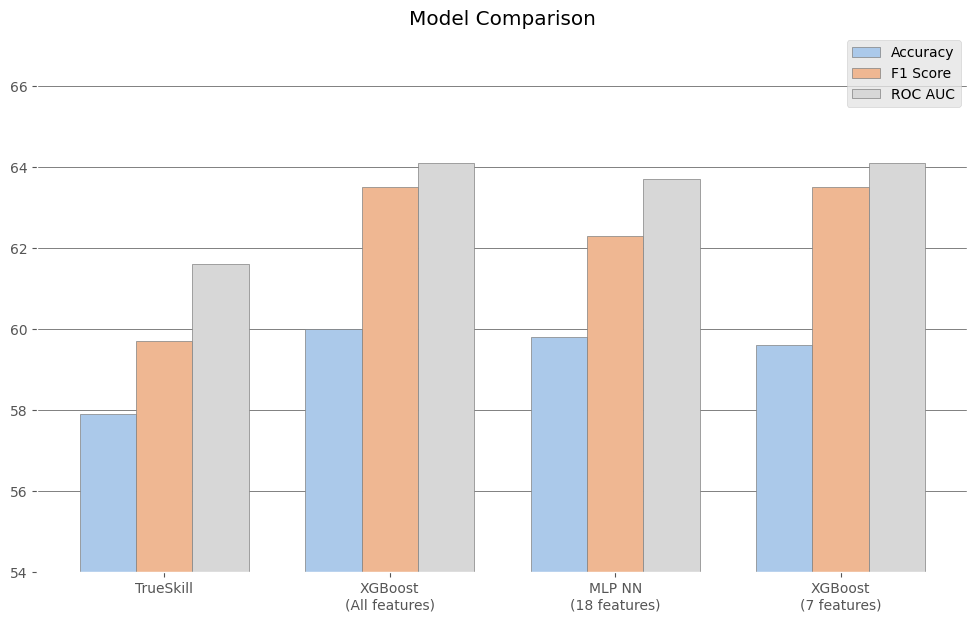
\includegraphics[width=1.1\textwidth]{Figures/results-bars.png}
	\end{adjustbox}
	\caption{Comparison of best accuracy, F1-score, and AUC ROC attained for models trained with different amounts of features}
	\label{fig:full-data-bars}
\end{figure}

\subsection{Filtered datasets}

\subsubsection{Excluding BO1 matches}

A common conception in the Counter-Strike community is that best-of-1 matches are more unpredictable and upsets are more likely. This is a reasonable expectation considering that fewer round wins are required to win the match, which can lead to more volatile outcomes. One would therefore expect an improvement in predictive accuracy when ignoring BO1 matches.

The dataset used for this analysis consisted of 8320 matches in total split using the same 80:20 ratio. 6656 matches were used to train the models, and their performance was evaluated by testing them on 1664 matches. The 18 selected features were determined using the feature importance graphs obtained earlier.

\begin{table}[h!]
	\centering
	\small
	\begin{adjustbox}{center} % Center the table
		\begin{tabular}{ |l|c|c|c|c|c|c| }
			\hline
			\rule{0pt}{2.6ex} \textbf{Model} & \textbf{Train ACC} & \textbf{Test ACC} & \textbf{Precision} & \textbf{Recall} & \textbf{F1 Score} & \textbf{ROC AUC} \\
			\hline
			\rule{0pt}{2.6ex} TrueSkill                 & 58.8 & 59.2 & 59.3 & 62.3 & 60.8 & 63.7 \\ \hline
			\rule{0pt}{2.6ex} Logistic regression       & 61.3 & 61.7 & 60.6 & 69.9 & 64.9 & 65.6 \\
			\rule{0pt}{2.6ex} Random forests            & 65.5 & 61.3 & 60.1 & \textbf{70.6} & 64.9 & 66.0 \\
			\rule{0pt}{2.6ex} Support vector machine    & 61.3 & 61.7 & \textbf{60.8} & 68.8 & 64.6 & 65.5 \\
			\rule{0pt}{2.6ex} XGBoost                   & 63.7 & \textbf{61.9} & \textbf{60.8} & 69.9 & \textbf{65.0} & \textbf{66.3} \\
			\rule{0pt}{2.6ex} Gaussian Naive Bayes      & 60.4 & 59.4 & 58.5 & 68.2 & 63.0 & 63.3 \\
			\rule{0pt}{2.6ex} Multilayer perceptron     & 62.1 & 61.1 & 60.2 & 68.8 & 64.2 & 65.9 \\
			\rule{0pt}{2.6ex} $k$-nearest neighbours 	& 61.2 & 60.9 & 59.9 & 69.2 & 64.2 & 65.7 \\
			\hline
		\end{tabular}
	\end{adjustbox}
	\caption{Performance of ML models trained with all features on dataset which excludes BO1 matches}
	\label{table:3}
\end{table}

The baseline TrueSkill model's classification accuracy improved slightly from 57.9\% to 59.2\%, a modest 1.3\% improvement. Almost all of models achieved over 60\% accuracy. XGBoost once again achieved the best performance, followed by SVM and logistic regression. These results empirically support the notion that Best-of-1's are more difficult to predict.

% Hyperparameters used
% LOG {'C': 1, 'penalty': 'l2', 'solver': 'liblinear'}
% RAN {'criterion': 'gini', 'max_depth': 5, 'max_features': 'log2', 'min_samples_leaf': 4, 'min_samples_split': 4, 'n_estimators': 300}
% SVM {'C': 0.1, 'gamma': 'scale', 'kernel': 'linear'}
% XGB {'learning_rate': 0.025, 'max_depth': 2, 'n_estimators': 200}
% GNV {'var_smoothing' : '1e-09'}
% MLP {'activation': 'tanh', 'alpha': 0.001, 'hidden_layer_sizes': (10,100,10), 'learning_rate_init': 0.001, 'solver': 'sgd'}
% KNN {'n_neighbors': 110, 'p': 1, 'weights': 'uniform'}

\subsubsection{LAN-only}

LAN tournaments are often prestigious events, and it is usually only the top teams who play in these matches. It is thus useful to understand the classification performance for these types of matches. Applying this filter reduces the number of matches significantly. Furthermore, in 2020 and a large part of 2021, almost no LAN matches were played due to the COVID-19 pandemic. The dataset therefore contains only 2130 matches, of which 1704 were used for training and 426 for testing. Note that these include all match formats, including BO1. 

\begin{table}[h!]
	\centering
	\small
	\begin{adjustbox}{center} % Center the table
		\begin{tabular}{ |l|c|c|c|c|c|c| }
			\hline
			\rule{0pt}{2.6ex} \textbf{Model} & \textbf{Train ACC} & \textbf{Test ACC} & \textbf{Precision} & \textbf{Recall} & \textbf{F1 Score} & \textbf{ROC AUC} \\
			\hline
			\rule{0pt}{2.6ex} TrueSkill                 & 54.8 & 59.9 & 59.0 & 64.8 & 61.7 & 62.8 \\ \hline
			\rule{0pt}{2.6ex} Logistic regression       & 58.1 & 60.1 & 59.6 & 62.4 & 61.0 & 63.5 \\
			\rule{0pt}{2.6ex} Random forests            & 63.8 & 62.4 & \textbf{61.4} & 67.1 & 64.1 & 63.9 \\
			\rule{0pt}{2.6ex} Support vector machine    & 58.0 & \textbf{62.7} & 61.1 & \textbf{70.0} & \textbf{65.2} & \textbf{64.2} \\
			\rule{0pt}{2.6ex} XGBoost                   & 67.2 & 60.3 & 59.7 & 63.4 & 61.5 & 61.8 \\
			\rule{0pt}{2.6ex} Gaussian Naive Bayes      & 57.0 & 59.9 & 59.5 & 61.5 & 60.5 & 61.7 \\
			\rule{0pt}{2.6ex} Multilayer perceptron     & 57.3 & 59.2 & 58.3 & 64.3 & 61.2 & 61.1 \\
			\rule{0pt}{2.6ex} $k$-nearest neighbours 	& 59.2 & 58.0 & 56.9 & 65.7 & 61.0 & 62.8 \\
			\hline
		\end{tabular}
	\end{adjustbox}
	\caption{Performance of ML models trained with selected features on dataset with only LAN matches included}
	\label{table:0}
\end{table}

SVM performed the best under these circumstances followed by random forests. XGBoost and the MLP did not perform as well as before. This was the first time an ML model achieved an accuracy in excess of 62\%. This dataset was, however, far smaller than the prior datsets. The best model achieved a 2.8\% improvement over the baseline TrueSkill model, which was more significant than previously obtained. These results empirically support the idea that LAN matches are more predictable than online matches.

% Hyperparameters used
% LOG {'C': 0.01, 'penalty': 'l2', 'solver': 'liblinear'}
% RAN {'criterion': 'gini', 'max_depth': 5, 'max_features': 'log2', 'min_samples_leaf': 4, 'min_samples_split': 4, 'n_estimators': 300}
% SVM {'C': 0.1, 'gamma': 'scale', 'kernel': 'linear'}
% XGB {'learning_rate': 0.025, 'max_depth': 2, 'n_estimators': 200}
% GNV {'var_smoothing' : '1e-09'}
% MLP {'activation': 'relu', 'alpha': 0.001, 'hidden_layer_sizes': (10,100,10), 'learning_rate_init': 0.001, 'solver': 'sgd'}
% KNN {'n_neighbors': 110, 'p': 1, 'weights': 'uniform'}

\subsubsection{Rating cut-off}

As discussed previously, the full dataset includes all matches played where at least one of the team's was ranked in the Top-50 on HLTV's world ranking. Does varying this constraint meaningfully impact the overall predictability of matches? To test this hypothesis, the rank threshold was adjusted to only consider matches played where at least one of the teams were ranked in the Top-30 and Top-15 respectively. The results are tabulated in Tables \ref{table:4} and \ref{table:5} below.

\textbf{Top-30}

This filter removed a sizeable number of matches from the dataset, leaving 7115 for analysis. 5692 were used for training the models and 1423 for testing.

\begin{table}[h!]
	\centering
	\small
	\begin{adjustbox}{center} % Center the table
		\begin{tabular}{ |l|c|c|c|c|c|c| }
			\hline
			\rule{0pt}{2.6ex} \textbf{Model} & \textbf{Train ACC} & \textbf{Test ACC} & \textbf{Precision} & \textbf{Recall} & \textbf{F1 Score} & \textbf{ROC AUC} \\
			\hline
			\rule{0pt}{2.6ex} TrueSkill 				& 57.4 & 58.0 & 57.8 & 62.4 & 60.0 & 61.5 \\ \hline
			\rule{0pt}{2.6ex} Logistic regression 		& 60.4 & 59.3 & 57.6 & 73.7 & \textbf{64.6} & 63.3 \\
			\rule{0pt}{2.6ex} Random forests 			& 62.9 & 58.1 & 56.6 & \textbf{73.0} & 63.7 & 61.7 \\
			\rule{0pt}{2.6ex} Support vector machine 	& 61.3 & 58.6 & 57.7 & 67.0 & 62.0 & 62.8 \\
			\rule{0pt}{2.6ex} XGBoost 					& 62.9 & \textbf{59.5} & 58.0 & 71.6 & 64.1 & \textbf{64.3} \\
			\rule{0pt}{2.6ex} Gaussian Naive Bayes 		& 58.2 & 57.2 & 57.8 & 56.3 & 57.0 & 60.8 \\
			\rule{0pt}{2.6ex} Multilayer perceptron		& 61.7 & 59.0 & \textbf{60.7} & 53.3 & 56.8 & 62.0 \\
			\rule{0pt}{2.6ex} $k$-nearest neighbours 	& 64.7 & 52.8 & 53.0 & 58.4 & 55.5 & 54.2 \\
			\hline
		\end{tabular}
	\end{adjustbox}
	\caption{Performance of ML models trained with selected features on dataset consisting only of Top-30 matches}
	\label{table:4}
\end{table}

The results obtained were very similar to the full dataset, with the baseline benchmark only improving its accuracy by 0.1\%. XGBoost and MLP once again proved to be the best performing models, which was expected given the earlier results. That being said, the best accuracy attained actually decreased slightly, from 59.8\% to 59.5\%.

\textbf{Top-15}

The ranking threshold was further constrained to only include matches with at least one Top-15 team. This dataset had 3756 matches, of which 3004 were used for training and 752 for testing.

\begin{table}[h!]
	\centering
	\small
	\begin{adjustbox}{center} % Center the table
		\begin{tabular}{ |l|c|c|c|c|c|c| }
			\hline
			\rule{0pt}{2.6ex} \textbf{Model} & \textbf{Train ACC} & \textbf{Test ACC} & \textbf{Precision} & \textbf{Recall} & \textbf{F1 Score} & \textbf{ROC AUC} \\
			\hline
			\rule{0pt}{2.6ex} TrueSkill 				& 58.2 & 58.5 & 59.3 & 62.6 & 60.9 & 61.6 \\ \hline
			\rule{0pt}{2.6ex} Logistic regression 		& 62.5 & 57.6 & 56.9 & 73.5 & 64.1 & 62.3 \\
			\rule{0pt}{2.6ex} Random forests			& 61.8 & 58.6 & 57.1 & \textbf{79.9} & \textbf{66.6} & 62.4 \\
			\rule{0pt}{2.6ex} Support vector machine 	& 63.3 & 58.1 & 57.0 & 77.1 & 65.5 & 63.7 \\
			\rule{0pt}{2.6ex} XGBoost 					& 66.5 & \textbf{62.0} & 61.8 & 69.1 & 65.2 & \textbf{65.8} \\
			\rule{0pt}{2.6ex} Gaussian Naive Bayes 		& 59.0 & 58.4 & \textbf{61.9} & 50.3 & 55.5 & 62.1 \\
			\rule{0pt}{2.6ex} Multilayer perceptron     & 64.4 & 60.2 & 59.5 & 71.9 & 65.1 & 61.9 \\
			\rule{0pt}{2.6ex} $k$-nearest neighbours 	& 66.3 & 51.6 & 52.7 & 61.3 & 56.7 & 54.0 \\
			\hline
		\end{tabular}
	\end{adjustbox}
	\caption{Performance of ML models trained with selected features on dataset consisting only of Top-15 matches}
	\label{table:5}
\end{table}

The results here mirror what was found with the LAN-only filter. Indeed, there is significant overlap between these two datasets, as teams which attend LAN events also tend to be higher-ranked. XGBoost obtained the highest classification ability once more, 62\%. It is noteworthy that each model (except Gaussian Naive Bayes) exhibited significantly better recall than precision. This means that the models tend towards positive classifications: true positives were often identified, however, more false positives also occurred.

One explanation for the improvement in model performance is that there is a greater proportion of mis-matches (Top-15 vs a lower ranked team) present in this subset of the data, which should be easier to predict.

\subsection{Summary}

Machine learning techniques outperform the baseline classification performance, albeit usually only by a few percentage points. XGBoost was found to consistently achieve better performance than the other methods employed, notably obtaining 62\% accuracy on the dataset which excluded BO1s. SVM and MLP also delivered good performance, sometimes beating XGBoost. In the LAN-only subset, SVM achieved 62.7\% accuracy.

The results suggest that LAN matches are more predictable than online matches, and that matches involving a higher-ranked team are generally easier to predict than a match with lower ranked teams. Additionally, BO3 and BO5 matches are easier to predict than BO1 matches.

Furthermore, it was found that incorporating many features did not measurably improve the predictive power of the models. Key features could be identified and selected using filter and wrapper techniques, but also from feature importance metrics produced by the models themselves. Training using a smaller subset of only the most relevant features reduced the tendency for models to overfit the training data while simultaneously reducing the computational requirements. These smaller models produced almost identical performance to the fully-featured models. 

\section{Betting odds and simulation}

The odds generated by the various models all exhibited a high correlation with the bookmaker odds, as shown in Table \ref{table:bettingperformance}. As explained in \ref{bettingstats}, the correlation, mean absolute error (MAE), and root-mean squared error (RMSE) for each model is reported. These measure the discrepancy between real odds offered by bookmakers and the odds generated by the models. Bet \% refers to the proportion of matches which were deemed to be worth betting on. The P/L column is the total number of betting units won or lost by the end of the betting period.

\begin{table}[h!]
	\centering
	\small
	\begin{adjustbox}{center} % Center the table
		\begin{tabular}{ |l|c|c|c|c|c|c|c| }
			\hline
			\rule{0pt}{2.6ex} \textbf{Model} & \textbf{Correlation} & \textbf{MAE} & \textbf{RMSE} & \textbf{Bet \%} & \textbf{Win \%} & \textbf{Loss \%} & \textbf{P/L} \\
			\hline
			\rule{0pt}{2.6ex} TrueSkill                 & 0.727 & 0.104 & 0.137 & 79.02 & 45.45 & 54.55 & -1.77 \\ \hline
			\rule{0pt}{2.6ex} Logistic regression       & 0.815 & 0.099  & 0.121 & 82.76 & 39.58 & 60.42 & 27.80 \\
			\rule{0pt}{2.6ex} Random forests            & 0.815 & 0.101 & 0.124 & 81.61 & 39.08 & 60.92 & 25.98 \\
			\rule{0pt}{2.6ex} Support vector machine    & 0.803 & 0.100 & 0.123 & 82.47 & 39.02 & 60.98 & 23.72 \\
			\rule{0pt}{2.6ex} XGBoost                   & \textbf{0.855} &  \textbf{0.088} & \textbf{0.108} & 81.90 & 38.60 & 61.40 & 21.38 \\
			\rule{0pt}{2.6ex} Gaussian Naive Bayes      & 0.774 & 0.102 & 0.135 & 80.17 & \textbf{51.25} &\textbf{ 48.75} & 15.27 \\
			\rule{0pt}{2.6ex} Multilayer perceptron     & 0.801 & 0.097  & 0.120 & \textbf{84.20} & 38.23 & 61.77 & 16.70 \\
			\rule{0pt}{2.6ex} $k$-nearest neighbours 	& 0.740 & 0.105 & 0.130 & 81.90 & 40.70 & 59.30 & \textbf{32.78} \\
			\hline
		\end{tabular}
	\end{adjustbox}
	\caption{Comparison of generated odds to real-world betting odds and per-model profit/loss}
	\label{table:bettingperformance}
\end{table}

The betting performance is of particular interest, as every ML model was profitable despite having a low percentage of winning bets relative to their classification accuracy. This counter-intuitive result is explained by the models assigning a higher probability (but still less than 50\%) to the underdog than what was implied by the bookmaker odds. The models effectively preferred to bet on the teams they predicted to lose. The large payouts from winning underdog bets offset the more frequent losses, resulting in an overall profitable strategy.

Every model considered over 80\% of the matches as worth betting on, with bookmakers offering favourable odds; odds for one of the teams being greater than what the model generated. The MLP produced the most avid betting activity, with 84\% of matches being bet on.

XGBoost, the model which repeatedly produced the most accurate classifications, shared the greatest overlap with the real-world odds, with a correlation of 0.855, MAE of 0.088 and RMSE of 0.108.

The most profitable model, $k$-NN, disagreed with the bookmaker odds the most; it had the lowest correlation of 0.740 and highest errors of all the ML models. 

The cumulative profit/loss for $k$-NN is plotted in Figures \ref{fig:profit-match} and \ref{fig:profit-date}. The first shows the profit/loss on a match-by-match basis, where the second shows the profit/loss with the date as the x-axis. The various horizontal lines in Figure \ref{fig:profit-date} are periods in which no matches were bet on. 

\begin{figure}[h]
	\centering
	\begin{adjustbox}{center}
		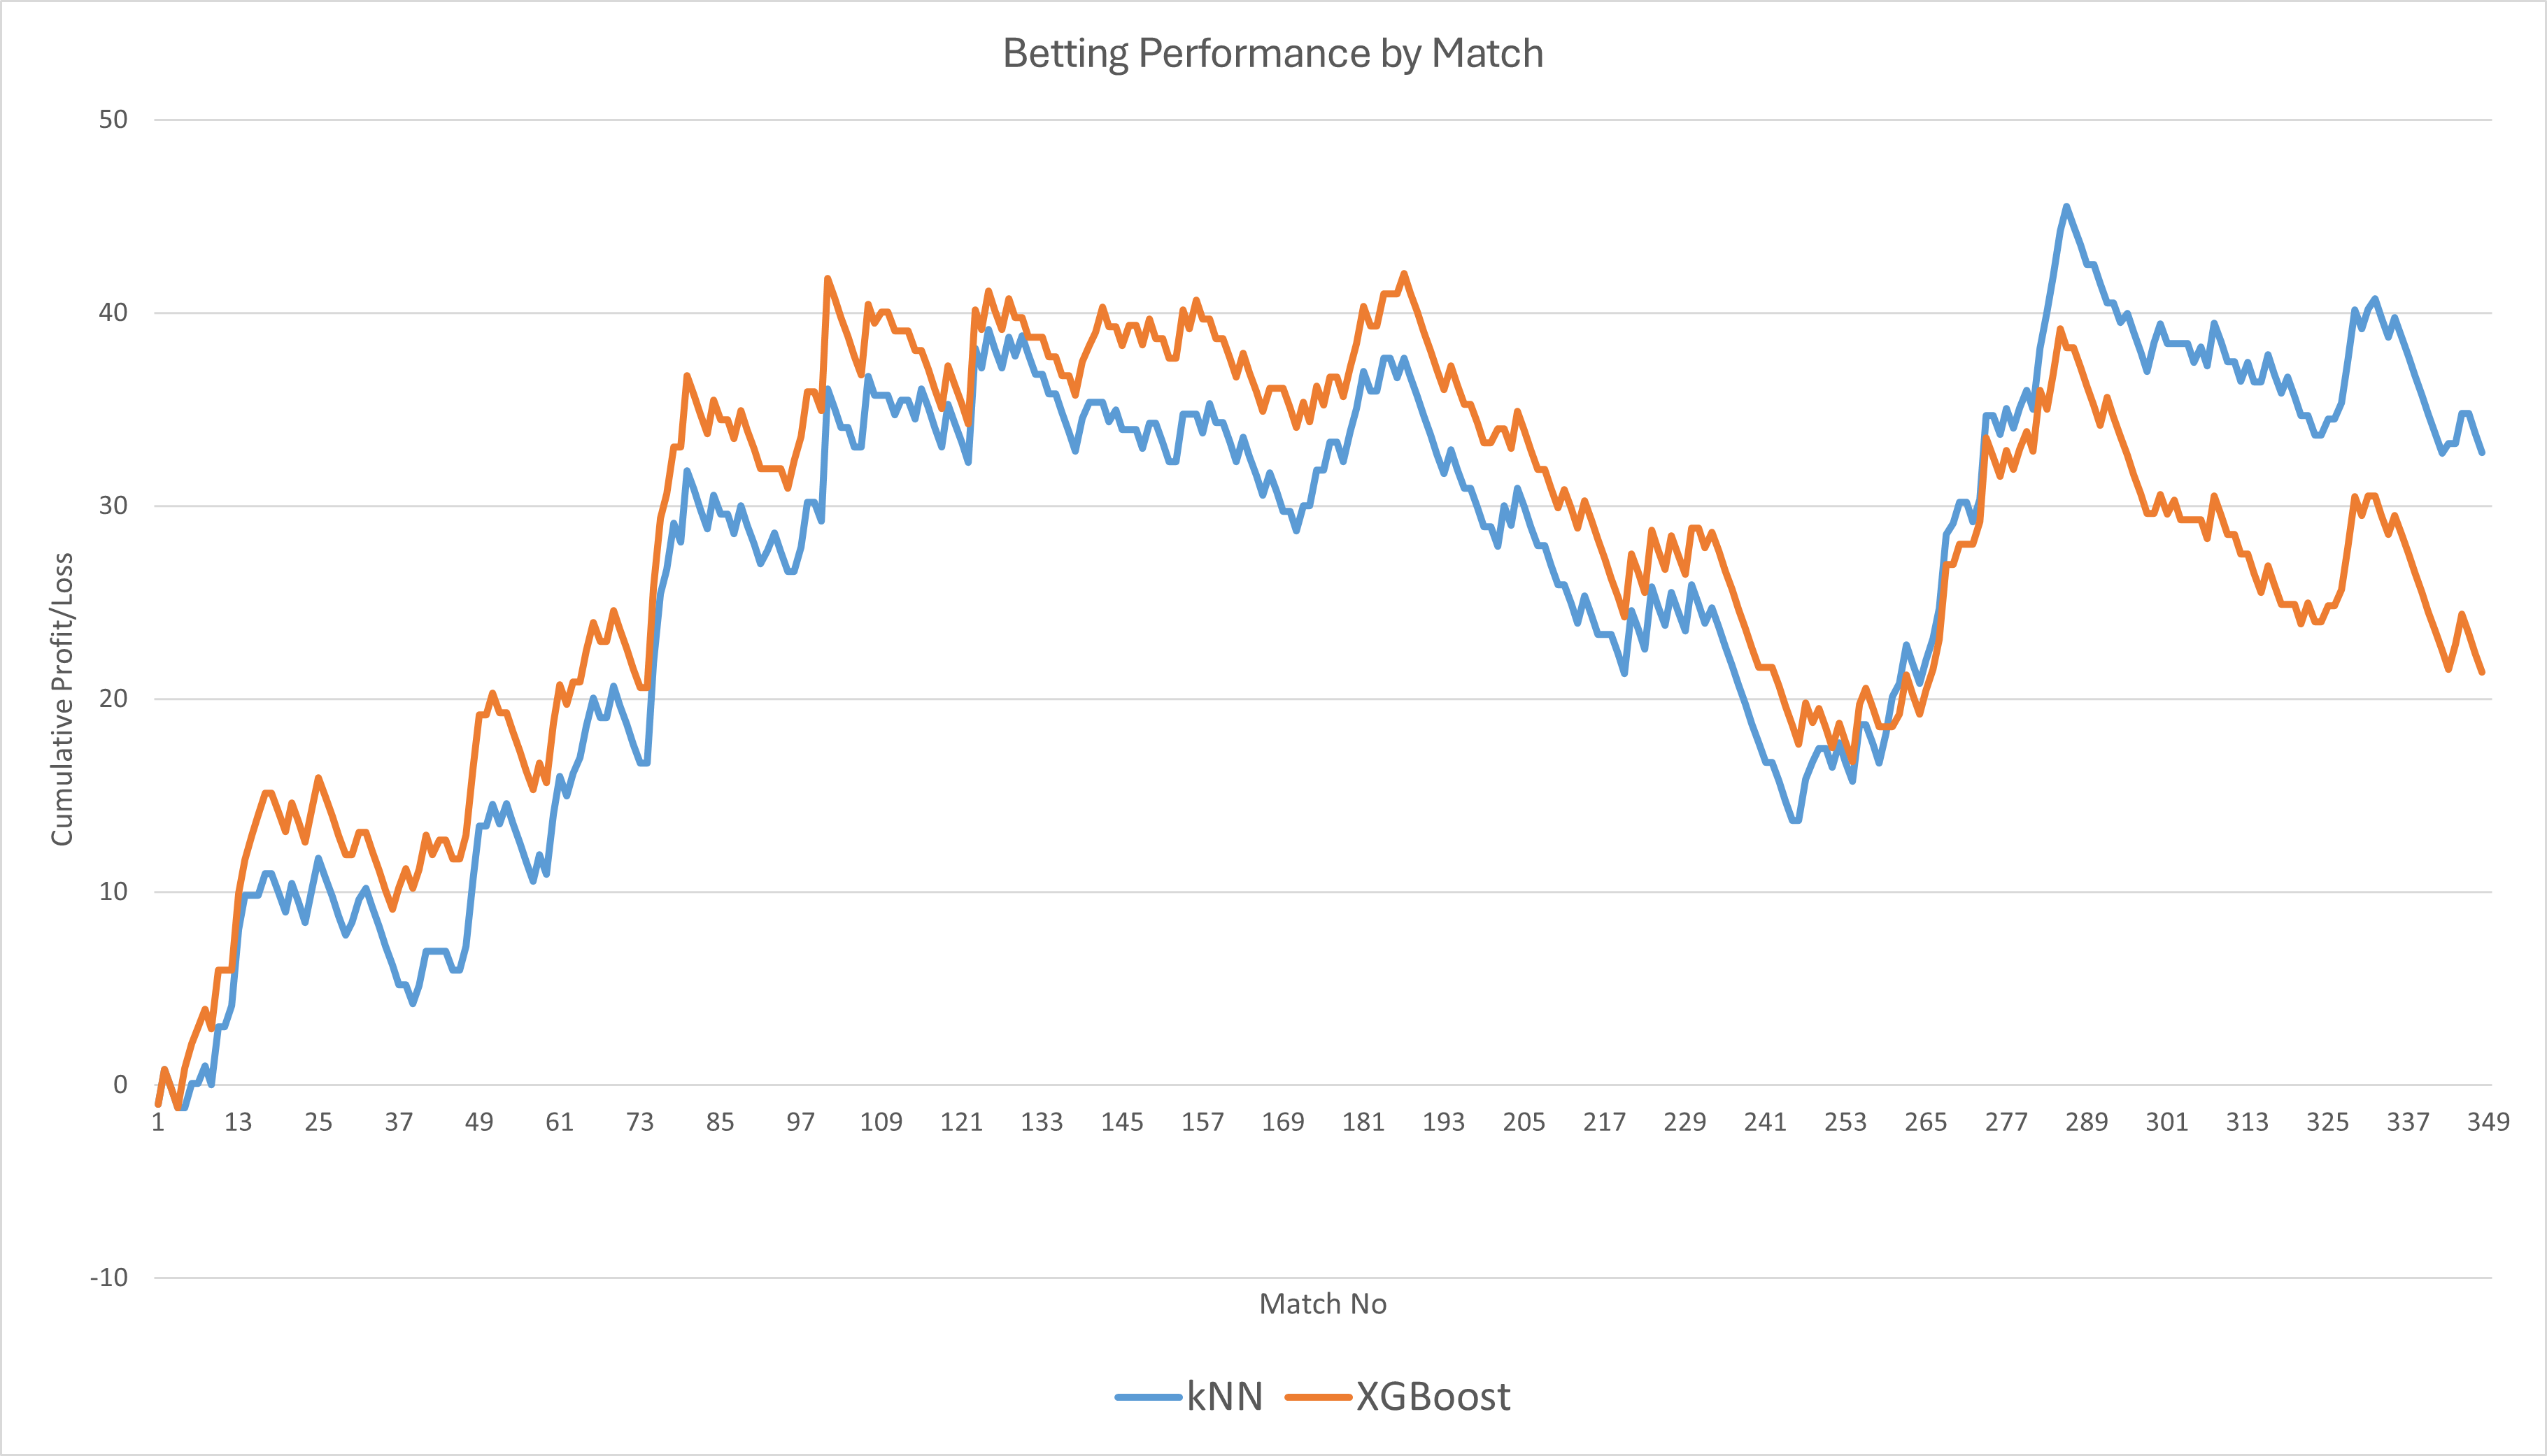
\includegraphics[width=\textwidth]{Figures/profit-match-2.png}
	\end{adjustbox}
	\caption{Cumulative profit/loss for $k$-NN and XGBoost (by match number)}
	\label{fig:profit-match}
\end{figure}

\begin{figure}[h]
	\centering
	\begin{adjustbox}{center}
		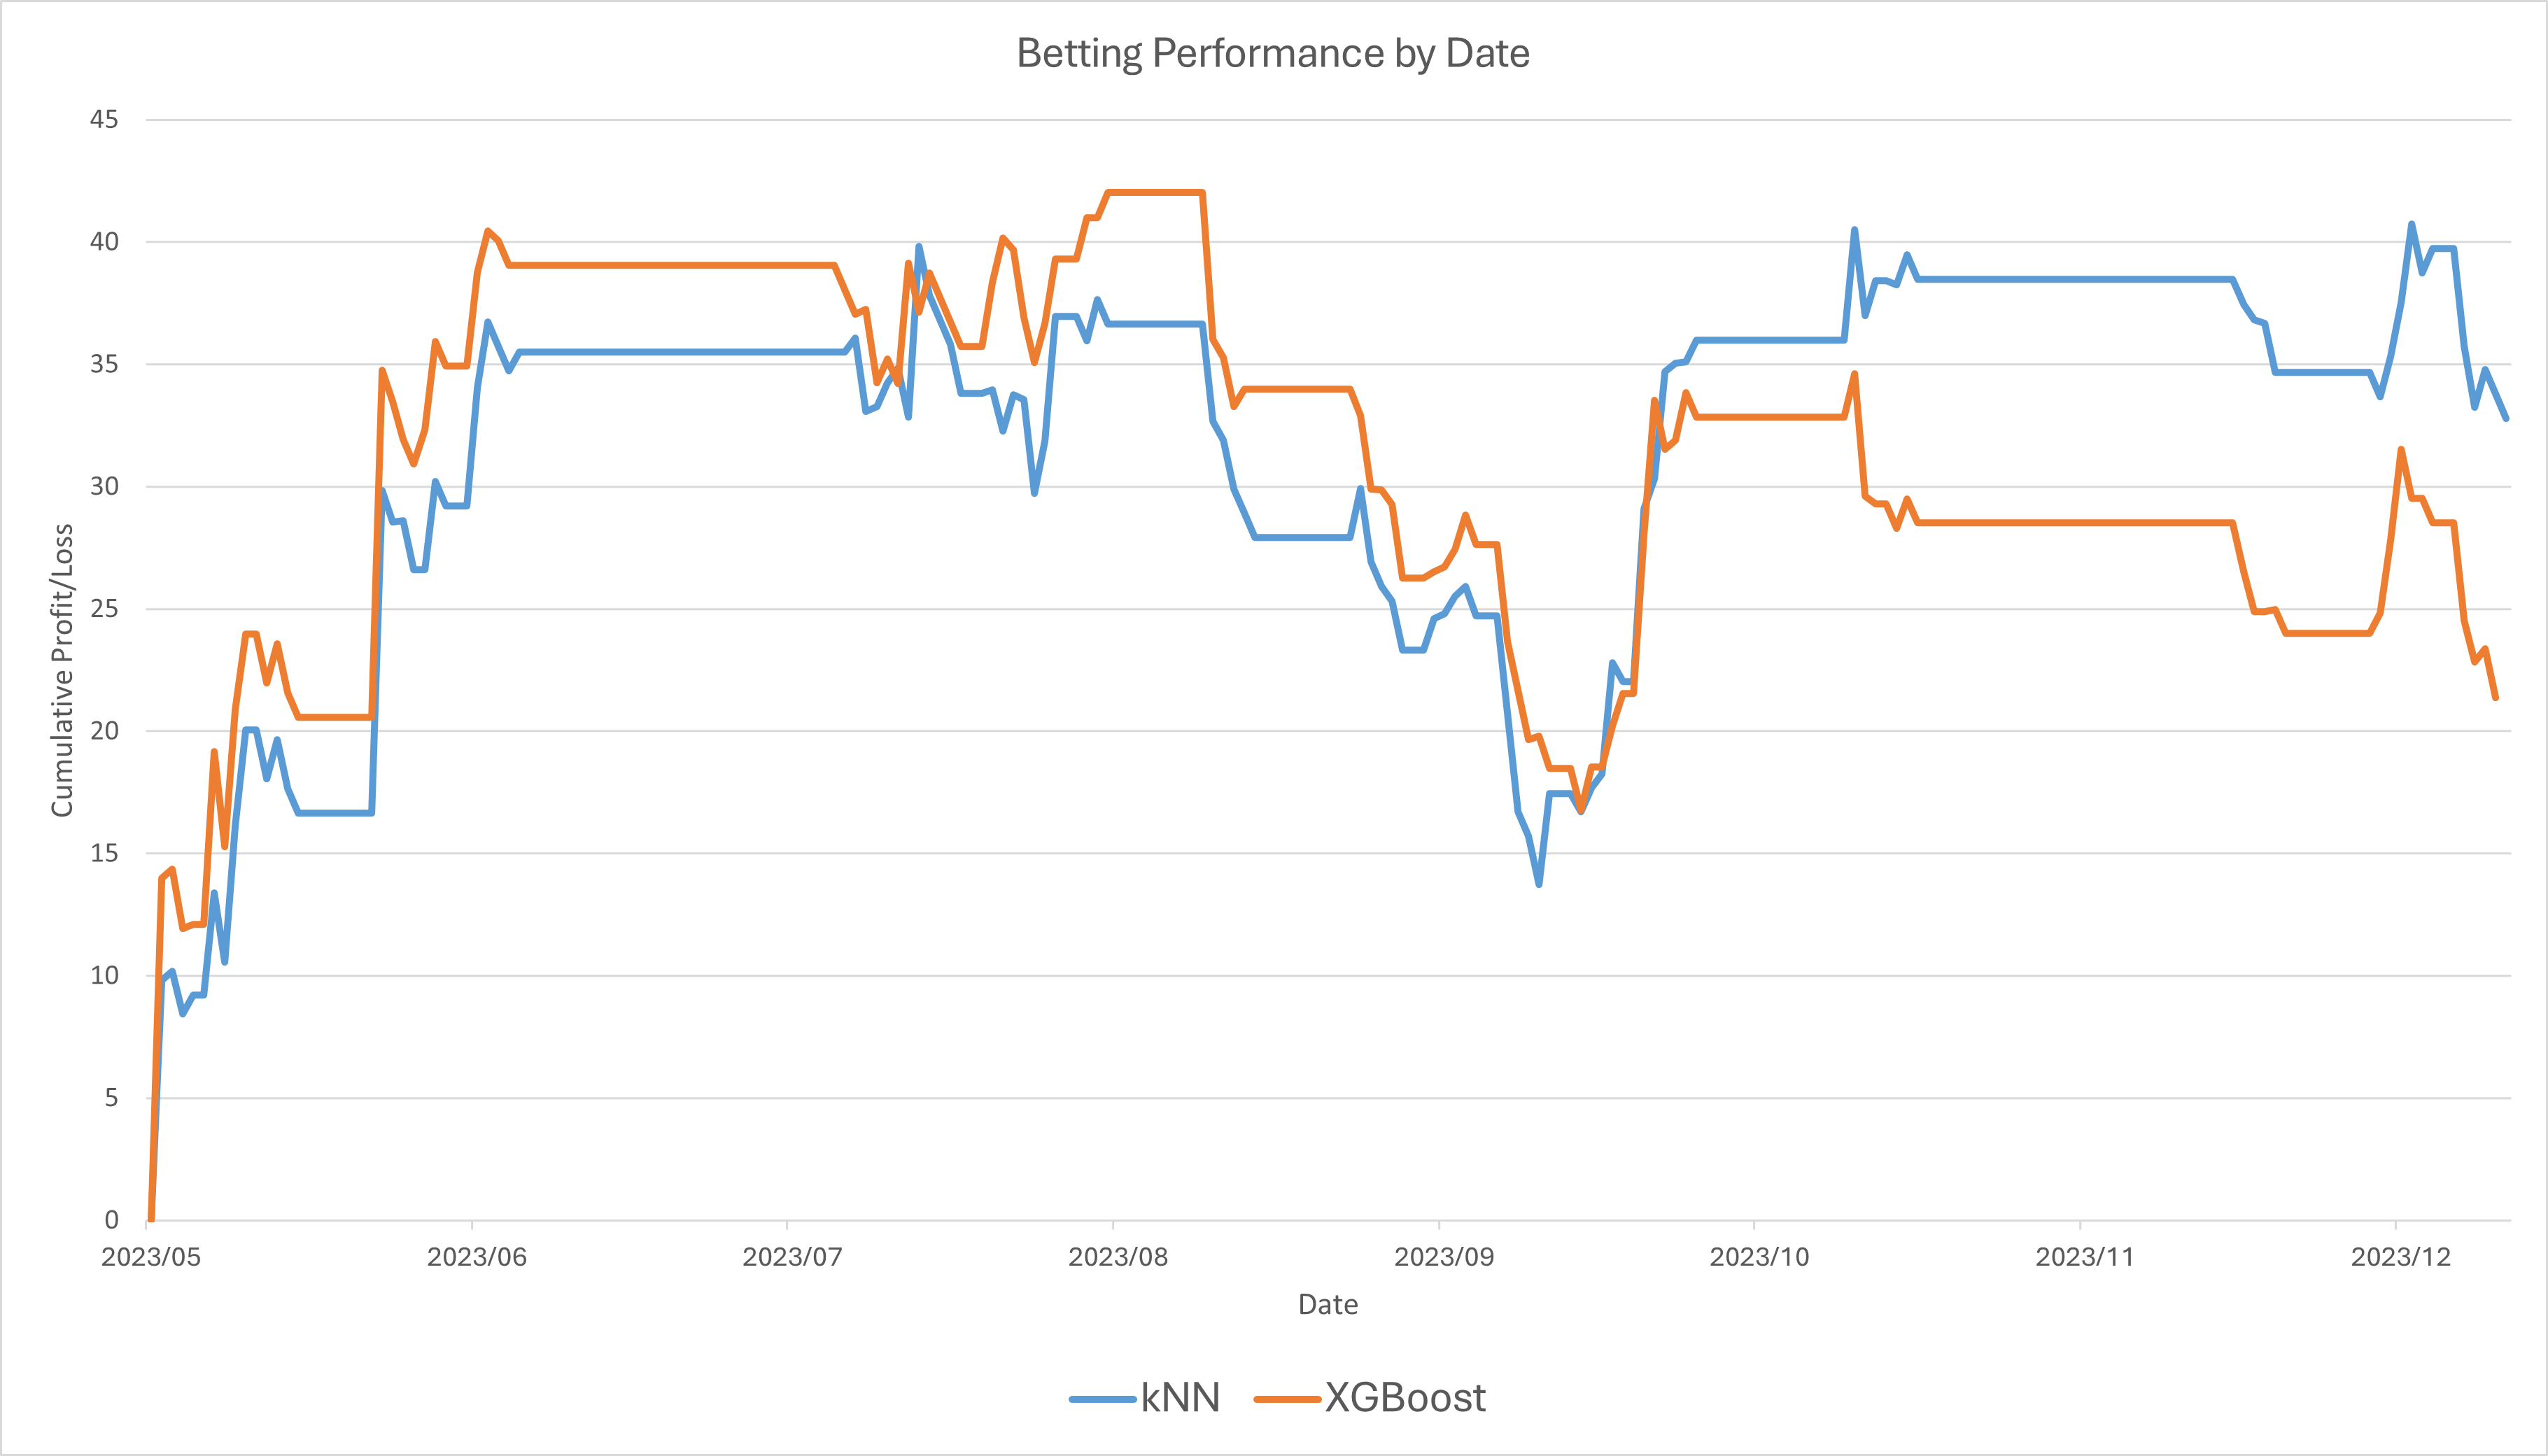
\includegraphics[width=\textwidth]{Figures/profit-date-2.png}
	\end{adjustbox}
	\caption{Cumulative profit/loss for $k$-NN and XGBoost (by date)}
	\label{fig:profit-date}
\end{figure}

It is interesting to note that the model which deviated most from the bookmaker odds was the most profitable. $k$-NN only shared a 74\% correlation with the bookmaker odds. The raw betting data for the $k$-NN model is included in the Appendix. It was found by observation that it would generate very high probabilities (>95\%) for teams more often than the other models, resulting in more "overdog" bets being placed. 

This was in contrast to the other, more accurate models which found most matches to be more balanced. In other words, these models often estimated the underdog as having a higher probability of victory than what the bookmaker odds suggested. They therefore placed underdog bets at a higher rate.

These results suggest that bookmaker odds exhibit some degree of bias which is exploitable. Over a relatively large sample size of matches (n=\matchesBet{}), the machine learning algorithms were all able to make a profit on the esports betting market by considering features generated from historical match data only. Further investigation into optimizing the betting strategy employed may yield even greater profits. 







